% GCM update: the five cases A-E. Redrawn after Fig. 3 of the article.
\documentclass[border=0pt]{standalone}
% Shared preamble of the GSO-RL documentation figures.
% Compiled with latex (DVI) + dvisvgm; see ../build.sh.
\def\pgfsysdriver{pgfsys-dvisvgm.def}
\usepackage[T1]{fontenc}
\usepackage{lmodern}
\renewcommand{\familydefault}{\sfdefault}
\usepackage{amsmath, amssymb}
\usepackage{tikz}
\usetikzlibrary{positioning, shapes, arrows.meta, calc, fit, backgrounds}

% Palette
\definecolor{Purple}{RGB}{102, 0, 153}
\colorlet{ColMa}{green!50!black}   % macro-move M1
\colorlet{ColMb}{blue!70!black}    % macro-move M2
\colorlet{ColMc}{orange!85!black}  % macro-move M3
\definecolor{cGa}{RGB}{38, 166, 154}
\definecolor{cGb}{RGB}{229, 96, 76}
\definecolor{cGc}{RGB}{235, 165, 40}
\definecolor{cGd}{RGB}{125, 125, 215}
\definecolor{cGe}{RGB}{190, 60, 150}

% White background so figures stay readable in dark mode. The white rectangle lives on the
% "background" layer; figures draw their own backdrops on "behind", which sits above it.
\pgfdeclarelayer{behind}
\pgfsetlayers{background,behind,main}
\tikzset{every picture/.append style={show background rectangle,
  background rectangle/.style={fill=white, draw=none}, inner frame sep=8pt}}
% NOTE: with dvisvgm, text placed after a \color{...} group inside the same node is misplaced.
% Put differently coloured pieces of text in separate nodes.

\newcommand{\yes}{{\color{green!50!black}\checkmark}}
\newcommand{\nope}{{\color{red!70!black}$\boldsymbol{\times}$}}

% A region: guide with three concentric rings.  \guia[style]{x}{y}{color}{label}
\newcommand{\guia}[5][]{%
  \fill[#4!10, #1] (#2,#3) circle (1.05);
  \fill[#4!20, #1] (#2,#3) circle (0.7);
  \fill[#4!35, #1] (#2,#3) circle (0.35);
  \foreach \r in {0.35,0.7,1.05} \draw[#4, #1] (#2,#3) circle (\r);
  \fill[#4!80!black, #1] (#2,#3) circle (2pt);
  \node[#4!75!black, font=\scriptsize\bfseries, #1] at (#2,#3+1.22) {#5};
}

\begin{document}
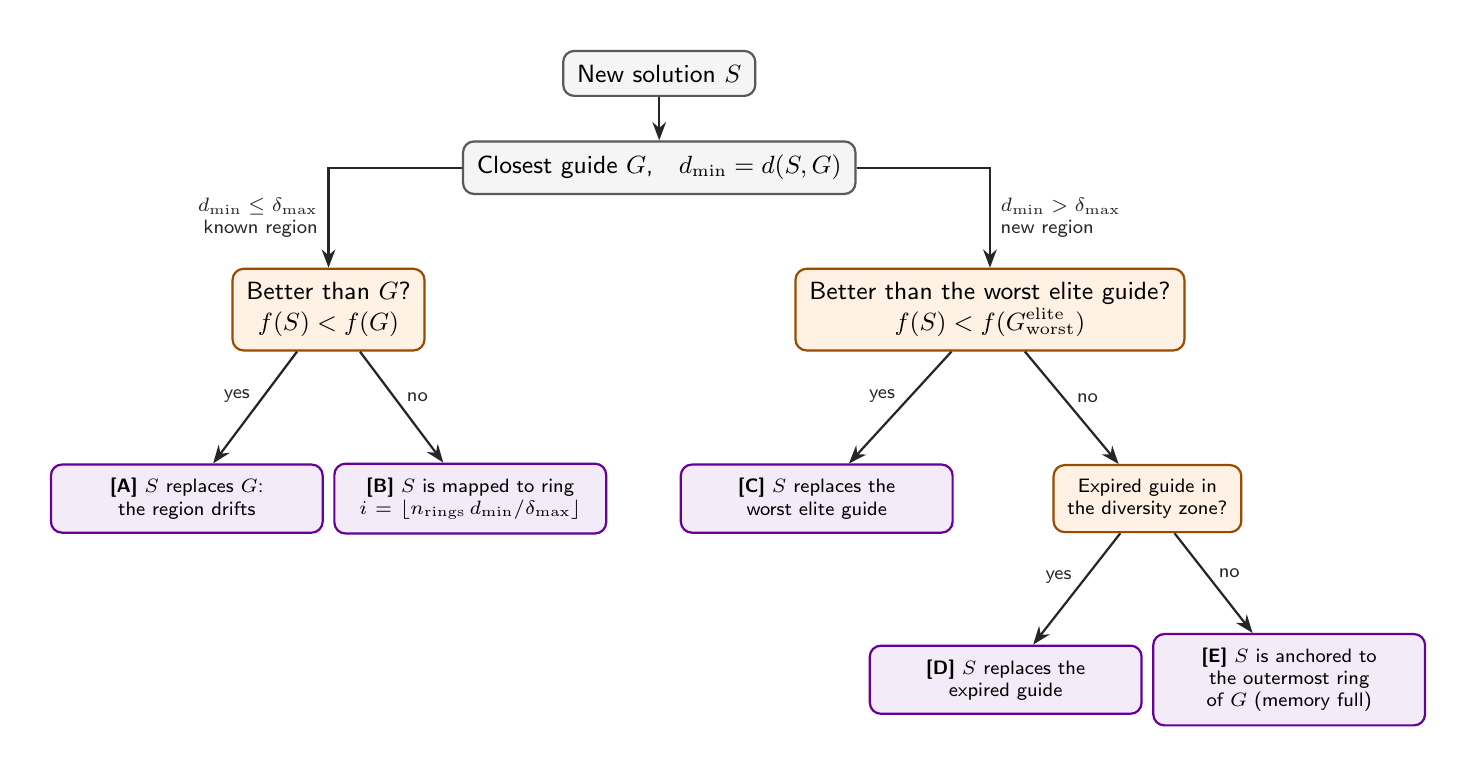
\begin{tikzpicture}[>=Stealth, font=\small,
  st/.style={rectangle, rounded corners, draw=gray!70!black, fill=gray!8, thick, align=center, inner sep=5pt},
  q/.style={rectangle, rounded corners, draw=orange!60!black, fill=orange!10, thick, align=center, inner sep=5pt},
  res/.style={rectangle, rounded corners, draw=Purple, fill=Purple!8, thick, align=center,
              text width=3.1cm, inner sep=5pt, font=\scriptsize},
  lab/.style={font=\scriptsize, fill=white, inner sep=1.5pt},
  arr/.style={->, thick, gray!30!black}]
  \node[st] (n) at (0,0) {New solution $S$};
  \node[st, below=0.55cm of n] (c) {Closest guide $G$,\quad $d_{\min} = d(S, G)$};

  \node[q] (k) at (-4.2,-3.0) {Better than $G$?\\ $f(S) < f(G)$};
  \node[q] (u) at ( 4.2,-3.0) {Better than the worst elite guide?\\ $f(S) < f(G^{\mathrm{elite}}_{\mathrm{worst}})$};

  \draw[arr] (n) -- (c);
  \draw[arr] (c.west) -| node[lab, pos=0.75, left=2pt, align=right] {$d_{\min} \le \delta_{\max}$\\ known region} (k.north);
  \draw[arr] (c.east) -| node[lab, pos=0.75, right=2pt, align=left] {$d_{\min} > \delta_{\max}$\\ new region} (u.north);

  \node[res] (A) at (-6.0,-5.4) {\textbf{[A]} $S$ replaces $G$:\\ the region drifts};
  \node[res] (B) at (-2.4,-5.4) {\textbf{[B]} $S$ is mapped to ring\\ $i = \lfloor n_{\mathrm{rings}}\, d_{\min} / \delta_{\max} \rfloor$};
  \node[res] (C) at ( 2.0,-5.4) {\textbf{[C]} $S$ replaces the\\ worst elite guide};
  \node[q, font=\scriptsize] (x) at (6.2,-5.4) {Expired guide in\\ the diversity zone?};
  \node[res] (D) at ( 4.4,-7.7) {\textbf{[D]} $S$ replaces the\\ expired guide};
  \node[res] (E) at ( 8.0,-7.7) {\textbf{[E]} $S$ is anchored to the outermost ring of $G$ (memory full)};

  \draw[arr] (k) -- node[lab, above left]  {yes} (A);
  \draw[arr] (k) -- node[lab, above right] {no}  (B);
  \draw[arr] (u) -- node[lab, above left]  {yes} (C);
  \draw[arr] (u) -- node[lab, above right] {no}  (x);
  \draw[arr] (x) -- node[lab, above left]  {yes} (D);
  \draw[arr] (x) -- node[lab, above right] {no}  (E);
\end{tikzpicture}
\end{document}
